\subsection{Selecting Target Stars (and Modelling Full Frame Images)}
\label{sec:selection_criteria}
For the Primary Mission, \tesss short cadence (2 min) targets will be drawn from a subset of the \tic. 
The prioritization statistic that the mission will use in this selection has yet to be explicitly defined.

We know that for \tess to detect small transiting planets
it should observe stars that are small and bright.  For this work, we
define a simple statistic, \texttt{Merit}, proportional to the SNR we
should expect from an arbitrarily sized planet orbiting any star:
\begin{align}
\texttt{Merit} &\equiv 
	\frac{1/R_\star^2}{\sigma_\text{1-hr}(I_c)/\sqrt{N_\text{obs}}}\ ,
\label{eq:merit}
\end{align}
where $R_\star$ is the radius of the star in question,
$\sigma_\text{1-hr}$ is the relative precision in flux measurements
over one hour of integration time, taken from an empirical fit to
Fig~\ref{fig:noise_with_moon}, $I_c$ is the Cousins band $I$ magnitude
\tess observes for the star (or more precisely, the star system) and
$N_\text{obs}$ is the number of observations the star receives over
the course of the mission.  For multiple star systems, $R_\star$ is
taken to be the radius of
the planet-hosting star, and the $I_c$ magnitude is computed from the 
combined flux of all the stars (this simulates contamination of the 
high-priority target list by the stars that have not been identified
as binaries).

\begin{figure*}[!tb] %[!thb]
	\centering
	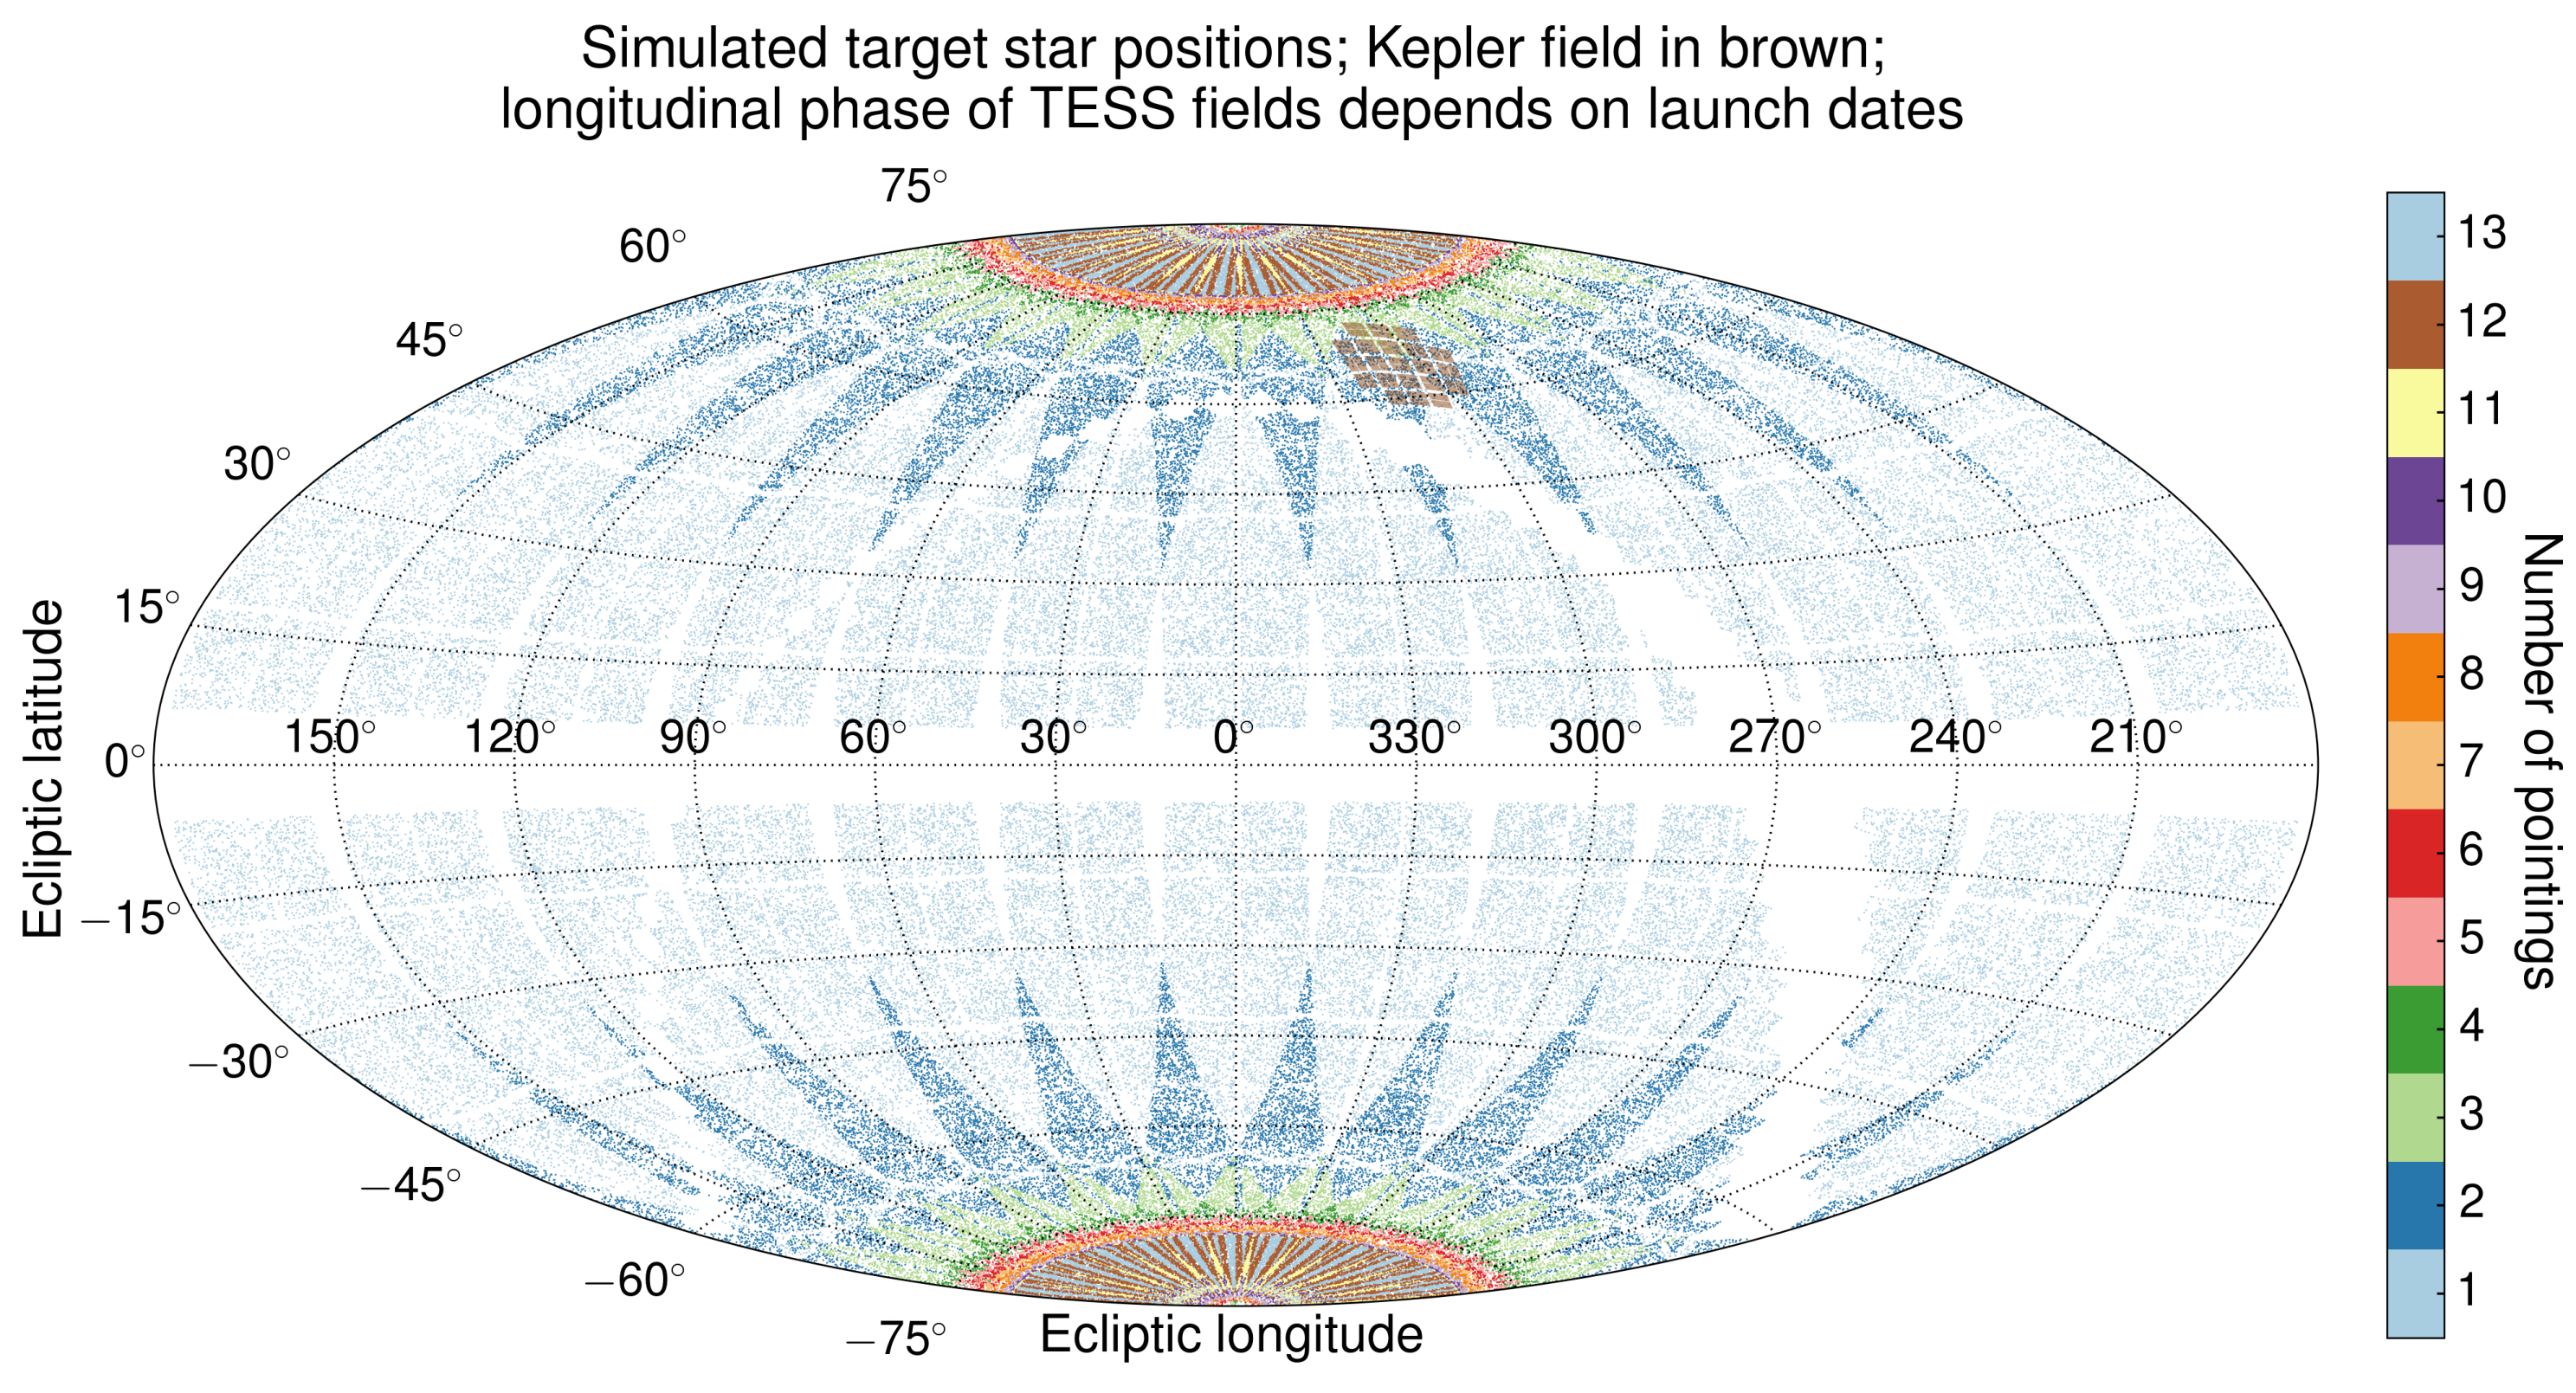
\includegraphics{figures/positions_pointings_kepler.pdf}
	\caption{Selected target stars in the Primary Mission. Their density 
	increases towards the poles because of the $\sqrt{N_\text{obs}}$ weight in 
	selection. Gaps in the focal plane array between each of a given camera's 
	four CCDs creates leads to the slight deviations from perfectly-continuous 
	observing shown at the ecliptic pole.}
	\label{fig:positions_pointings}
\end{figure*}
\begin{figure}[!tb] %[!thb]
	\centering
	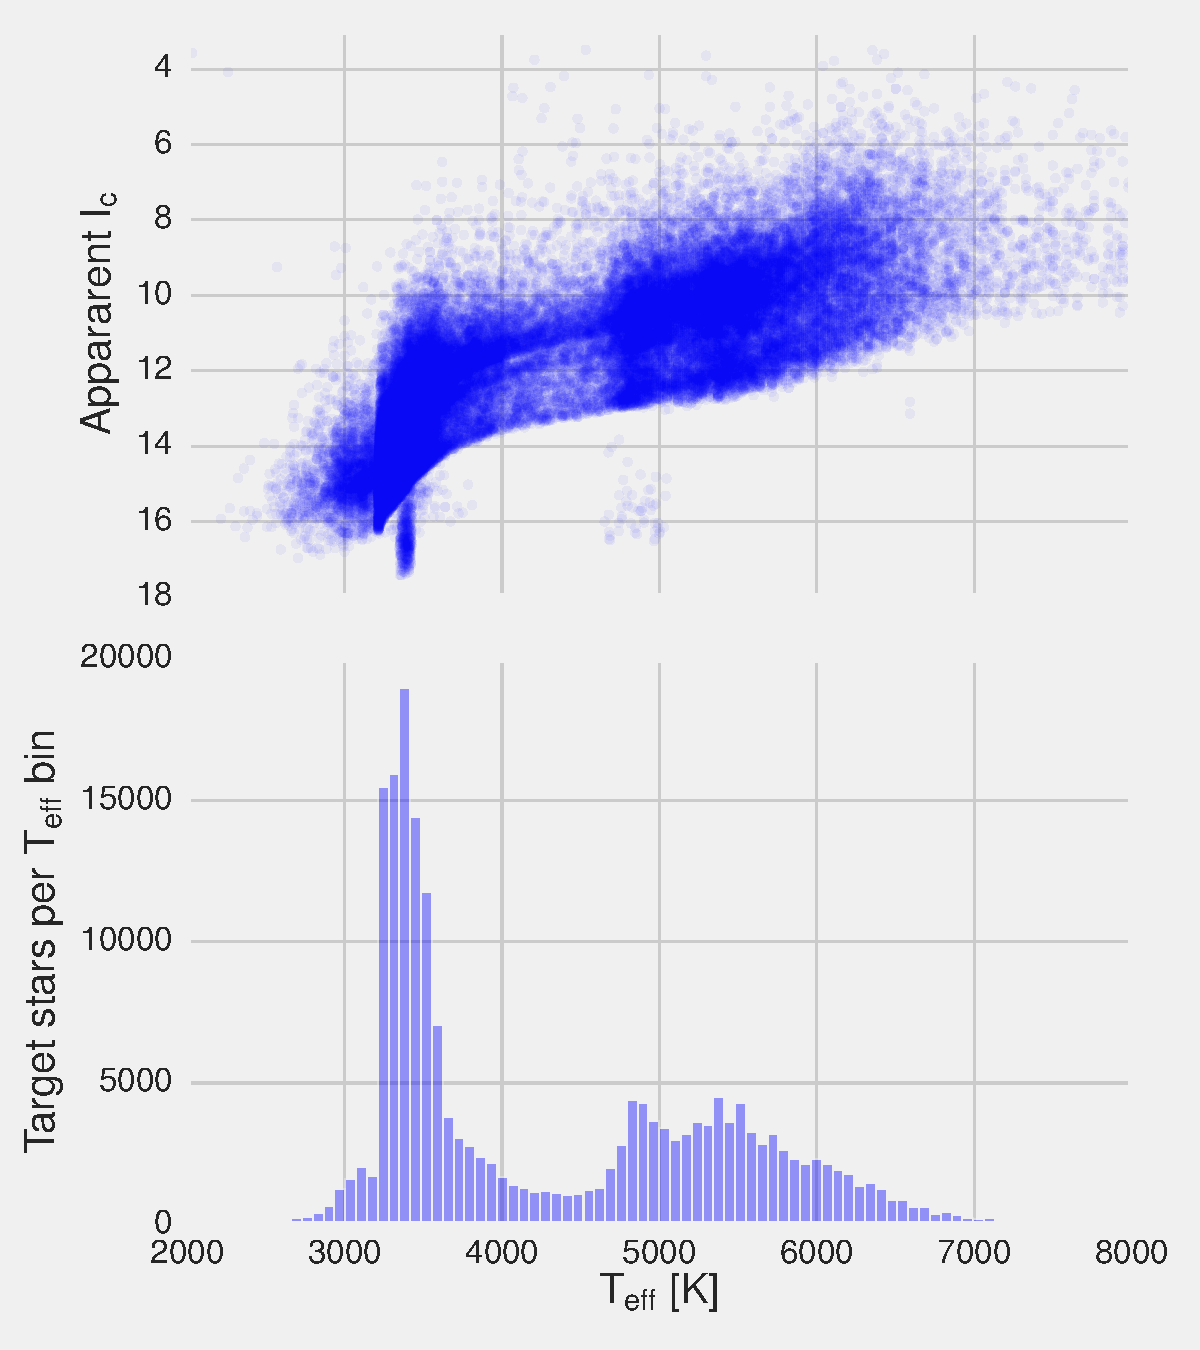
\includegraphics{figures/fig17_replica.pdf}
	\label{fig:fig17_replica}
	\caption{Target star Cousins I magnitude against effective temperature 
		(replicates Figure 17 of~\protect\citetalias{Sullivan_2015}). 
		Target stars are selected as the best $2\times10^5$ stars according to $\texttt{Merit}\equiv \sqrt{N_\text{obs}}(1/R_\star^2)/\sigma_\text{1-hr}(I_c)$. 
		The top subplot shows 1 in 10 stars. This simple model could inform the target selection to be performed on the \tic. 
		The lower histogram is bimodal, selecting heavily for M
		dwarfs, and selecting more F and G dwarfs than K dwarfs. This
		shape arises from the combined $1/R_\star^2$ and
		$1/\sigma_\text{1-hr}(I_c)$ weights: the fact that the minimum
		falls around K dwarfs occurs because of both a Malmquist bias
		(there are more F than K stars of comparable brightness in our
		catalog from which to select) as well as a corresponding dip
		in the TRILEGAL (\& observed) $V$-band luminosity functions
		(see~\citetalias{Sullivan_2015} Figure 5).
		% N.b. Winn showed this bias ANALYTICALLY in the searchable stars memo (he showed there are ~4* more stars e.g. in 0.75<R/Rsun<0.85 than 0.5<R/Rsun<0.6)
		
		Outliers visible in the upper scatterplot are non-physical,
		possibly artifacts from~\citetalias{Sullivan_2015}'s
		Padova-to-Dartmouth interpolation as they tend to have greater
		masses than all other stars on the main sequence. 
		As they comprise less than 1\% of the target stars, we ignore them
		in order to proceed.
		%Outliers in the upper scatterplot are almost certainly non-physical, but are less than 1\% of the catalog. Call it `sloppy' but I can show you a bunch of plots that make me think this is~\citet{Sullivan_2015}'s Padova-Dartmouth replacement scheme gone awry. Maybe it was bad interpolation.
		%\todo[inline]{reword snarky paragraph}
		% Q: could these just be in the CVZs? A: no. A much larger proportion are actually close to the ecliptic, which suggests a bias that I don't understand. An above-average fraction are in binary systems, but I don't have easy access to the binary companions.
		% Well, what are they? I think it might have something to do with the weird, likely non-physical (perhaps imposed by Peter's mass/radius fiddling) split you see in the Fig16 replica that you're not showing here.
		% Why? See our replica of Fig4, showing the nasty things that happen with EB radii + different radius / luminosity tracks being all mixed together!!
		% This would be important to address if it were the main focus.
		% Even though it looks ugly it's only ~700 stars. This means it's a ~1 % effect. Consequently, I'm fine with ignoring it.
	}
\end{figure}
\begin{figure}[!tb]
	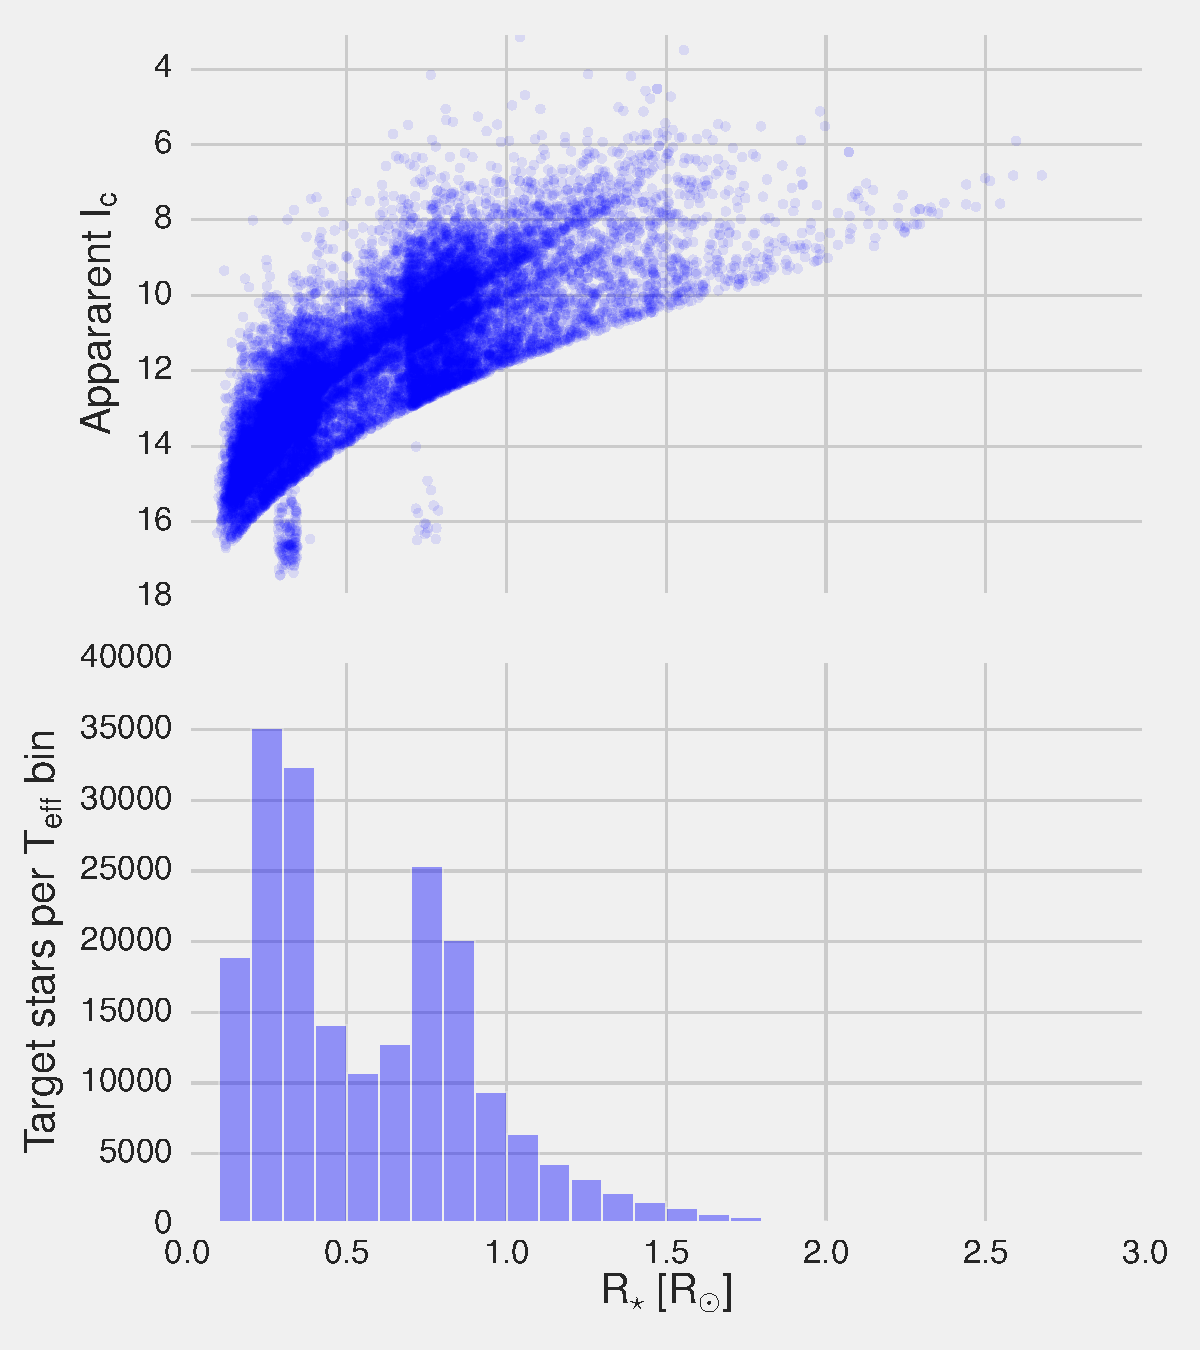
\includegraphics{figures/fig17_radius_on_x.pdf}
	\label{fig:fig17_radius_on_x}
	\caption{Same as Fig.~\protect\ref{fig:fig17_replica}, but as a function of stellar radius. $1/R_\star^2$ selection weight clearly visible, along with the same outliers.
	}
\end{figure}


We evaluate \texttt{Merit} for all the star systems in our modified
TRILEGAL catalog, and then choose the highest-\texttt{Merit} 
$2\times10^5$ as target
stars to be observed at 2 minute cadence.  Target stars selected in
this manner are shown in Fig.~\ref{fig:positions_pointings}. 
This statistic is simpler than the procedure outlined in Section 6.7
of~\citetalias{Sullivan_2015} and it produces a nearly identical
population of target stars (shown in Fig~\ref{fig:fig17_replica}).
Our approach for full frame image simulation is different from that
of~\citetalias{Sullivan_2015}, and we describe it below.

We generalize our \texttt{Merit} statistic to Extended Missions as 
follows: over an
entire mission, the total number of observations a star receives is
the sum of its observations in the Primary and Extended Missions:
$N_\text{obs}=N_\text{primary}+N_\text{extended}$.  If
$N_\text{extended}=0$ for a given star, then do not select that star as a
target star in the Extended Mission.  Else, compute its \texttt{Merit}
(Eq.~\ref{eq:merit}) substituting
$N_\text{obs}=N_\text{primary}+N_\text{extended}$.  In this manner
stars that are observed more during the Primary Mission are more
likely to be selected during the Extended Mission.
 

\paragraph{Alternative prioritization approaches:}

It is worth emphasizing that our scheme for selecting target stars for
an Extended Mission does not make use of any information on whether
candidate transit events were detected during the Primary Mission.  If
a star were observed at short cadence for an entire year, and no
candidate events were found, it might be sensible to disregard that
star in the Extended Mission in favor of stars that have never been
observed at short cadence -- particularly those with candidate events
that were detected in the Primary Mission full-frame images.  These
and related concerns are discussed further at the accompanying Wiki
document\textsuperscript{\ref{fn:wiki}}.

More abstractly, the procedure of simply applying Eq.~\ref{eq:merit}
attempts to select a stellar sample that will yield the most small
transiting planets around the brightest stars.  An alternative
approach would be to select stars that will give the most 
\textit{relative benefit} in 2 minute postage stamps over 30 
minute cadence observations since all stars will be present in the
30 minute images.  This `relative benefit' could be based on
improvement in transit detectability, or perhaps improved 
capacity to resolve the partial transit phases.

For purposes of transit detection, the difference between 2 and 30
minute cadence matters most when transits have short durations -- in
other words for small stars, and for close-in planets.  Switching to
this alternative approach would consequently bias us even more
strongly towards selecting M dwarfs.  We already select almost every M
dwarf with $I_c < 14$.  The limiting $I_c$ magnitude for detecting
$R_p > 4R_\oplus$ planets with \tess is $\sim\!16$, which is where we
see the dimmest stars in Fig.~\ref{fig:fig17_replica}.

Additionally, the procedure of applying Eq.~\ref{eq:merit} and
assuming that it will maximize the number of small planets that \tess
will detect about bright stars ignores the functional dependence of
planet occurrence rates on stellar properties.  For instance, should
we prioritize target stars that are metal-rich?  Metal-rich stars
demonstrably host more giant planets within \tesss period sensitivity
than metal-poor
stars~\citep{fischer_planet-metallicity_2005,johnson_giant_2010}.  The
question of whether this correlation extends to sub-Neptune radius
planets is somewhat contested, but for
instance~\citet{wang_revealing_2015} used a sample of KOIs and found
that the planet occurrence rates of (gas dwarf) planets are
$1.72^{+0.19}_{-0.17}$ ($2.03^{+0.29}_{-0.26}$) higher around
metal-rich than metal-poor stars.  Note that in this study,
`terrestrial' means $R_p<1.7R_\oplus$, `gas dwarf' 
$1.7R_\oplus < R_p < 3.9R_\oplus$, and the authors focused only on
solar-type stars ($4800\ \mathrm{K}<T_\mathrm{eff}<6500\ \mathrm{K}$).

A more robust approach for \tesss target selection might take these
kinds of results into account probabilistically.  For
instance,~\protect\citet{kipping_transit_2016} note that the
probability of short-period transiters having additional transiting
outer companions is functionally dependent upon the properties of the
short period transiters -- for instance their orbital periods and
radii.  They navigate the optimization problem using artificial neural
networks (ANNs) trained to select for features that improve the
probability of detecting transiting outer companions.  \tess might
benefit from a similar approach in target selection.

\paragraph{Alternative prioritization approaches in Extended Missions:}
Our \texttt{Merit} statistic also neglects the possibility of an Extended
Mission which only observes stars with known planets or planet
candidates (\tesss objects of interest, or those from other transit
and RV surveys) at short cadence.  This approach would free up a
considerable portion of \tesss data mass for full frame images at
\textit{e.g.}, 15 minutes rather than the current nominal 30 minutes.

\paragraph{Approach to full-frame images:}
\label{sec:FFI_simulation}
We want to simulate the full frame image detections in a
computationally tractable manner.  While~\citetalias{Sullivan_2015}
evaluated the phase-folded SNR for every potentially transiting object
about each of the $\sim\!1.6\times10^8$ stars in our synthetic catalog,
we focus only on the stars for which \tess could plausibly detect a
sub-Neptune planet over the 3-year mission.  Most stars that
\tess sees are too dim or too large to detect $R_p<4R_\oplus$ planets
-- while we expect many giant planet detections towards the galactic
plane (\citetalias{Sullivan_2015} Fig 19), small-planet detections are
more nearly isotropic, since practically all occur for stars at
$<1\rm\ kpc$.  For our purposes in this study, we argue that knowing
there will be thousands of giant planet candidates is sufficiently
accurate. The prospects for detecting smaller planets are more likely
to help discriminate between different scenarios for the Extended Mission.

In this vein, we only simulate full frame image detections for the
$3.8\times10^6$ highest \texttt{Merit} stars following the
$2\times10^5$ highest \texttt{Merit} stars observed as `postage
stamps'.  This number ($3.8\times10^6$) was initially estimated based
on the number of searchable stars about which we expect \tess to be
able to detect sub-Neptune radius
planets~\citep{winn_searchable_2013}.  The detection process is then
identical to that for postage stamps, except with 30 minute instead of
2 minute exposures, which increases the apparent durations and shrinks
the apparent depths for transits with durations of $\lesssim 1$ hour.

To check that the $4\times10^6$ highest \texttt{Merit} stars includes 
all stars about which \tess might detect sub-Neptune radius planets, 
we repeated this process for the Primary Mission using $5.8\times10^6$,
$9.8\times10^6$ and $19.8\times10^6$ `full frame image' stars, and
confirmed that there was no significant difference in the planet
yields at $R_p\le4R_\oplus$ between any of the cases.
%see ext_sim_notes/160817_on_the_FFI_assumtion. (10 Monte Carlo realizations each)
Increasing the number of FFI stars, the runs yield
increasing numbers of giant planets, particularly near the galactic
disk.  Meanwhile the number of sub-Neptune radius planets remains
fixed, and thus convinces us that our simulation includes a sufficient
number of target stars to be complete for sub-Neptune detection statistics.
